\chapter{Evaluation}
\label{chap:Evaluation}
\renewcommand{\arraystretch}{0.5}

In this chapter, we will go through our experimental hypotheses, testing scenarios, experiments conducted on two sample 
stereo matching algorithms, SGBM and ADCensus, and the results with our
proposed evaluation system to assess the benefits of using our evaluation model for outdoor AR applications over the general-purpose evaluation models; 
the Middlebury and Kitti Stereo Evaluation.

\section{Stereo Dataset}
It should be noted that the stereo images we have used to conduct the experiments on stereo algorithms in our system,
are selected from Kitti Stereo Dataset.
In contrary to the Middlebury dataset, Kitti Stereo Project provides stereo images and ground truth disparity maps
that are taken from outdoor scenes under real circumstances. This property of sample images makes them more appropriate 
for evaluating the performance of the algorithms in outdoor AR applications, thus better meeting the objectives of this study.
We have selected 52 image pairs from the Kitti Stereo dataset based on different photometric and visual properties that are important
in stereo vision and an AR application. Some 
of these properties are listed as follows:
\begin{itemize}
\item Light and shading; that is the scenes including bright, dim, and dark regions
\item Various depth ranges; that is including near field, medium field and far field objects  
\item Depth discontinuity and occlusion
\item Well textured and textureless regions
\end{itemize}


\section{Methodology}

Before going through the explanation of the experiments conducted to assess our evaluation model, we restate our main research question in this
study to better justify our hypotheses and the experiments defined for their validation. 
As mentioned earlier in chapter \ref{chap:Introduction}, our main objective is to investigate whether using 
stereo matching techniques to generate the depth map of the 
surrounding environment in an outdoor AR application can meet the requirements of the AR system. 
Therefore, our experiments focus 
on assessing those aspects of our evaluation model that assist to better answer this question.
As a result, our first attempt towards evaluating our model is to investigate and demonstrate whether the results of the evaluation process 
are properly measured and presented in the framework of the important factors in an outdoor AR application.
After confirming this property, which is the key property of our model, we investigate the effect of our proposed masking 
approach on the evaluation results. Moreover, we present how the methods are evaluated in the framework of 
real-time interactive AR systems.
We also explain how the evaluation and comparison of the methods is done in our model through some
experiments on the sample stereo matching algorithms.

\section{Hypotheses}

We have defined a set of hypotheses to evaluate our proposed design. These hypotheses are as follows:

\begin{itemize}
\item \textbf{Hypothesis 1}: \emph{Our model evaluates and demonstrates the performance of the stereo matching algorithm in the framework of 
outdoor augmented reality applications.} 
Unlike the Middlebury and Kitti benchmarks which are considered general-purpose evaluation models, 
our system can particularly evaluate the algorithms in the framework of an 
outdoor augmented reality application to facilitate the process of determining
the proper method for using in the AR system for a high quality real-time generation of the depth map of the surrounding environment from 
the user's point of view.

\item \textbf{Hypothesis 2:} \emph{Observing, evaluating, and consequently 
refining the areas near the depth edges in an image are more important in an AR application.}
Salient edges caused by depth discontinuities, 
which can also represent the object boundaries and occlusion, are one of the 
most important depth cues that helps the observer to better perceive the depth of different objects in the scene. In other words, the areas near the edges corresponding to depth discontinuities
in a scene are more important to the human visual system for perception of depth in an AR application and therefore, the disparity 
errors in these regions can be detected easier by the HVS. Therefore, we argue that in our model, the evaluation of the disparity results in these regions can be of great value 
to an outdoor AR application.

\item \textbf{Hypothesis 3:} \emph{Our system is better than other evaluation models for assessing the performance of the algorithm in
eal-time AR applications.}
Other evaluation models, the Kitti and Middlebury benchmarks, do not evaluate and report on the efficiency of the algorithms
with respect to their execution time. On the other hand, our system is capable of examining and evaluating an algorithm 
based on its execution time and therefore, can report its efficiency for real-time AR applications.

\end{itemize}

The experiments designed to validate these hypotheses are explained in the following sections.

\section{Experimental Environment and Settings}
Experiments were carried out on a Linux machine with Intel Core(TM) i7 3.20GHz CPU. 
Although ADCensus is proposed as a GPU-based solution to the problem of stereo correspondence, 
we have used the CPU implementation of both algorithms in all the experiments.
The set of parameters used at different steps of the evaluation are presented in the following sections.
It should be noted that these parameters were kept constant for all the images and experiments. However, if a parameter is changed during an experiment for certain
reasons, it will be explicitly mentioned in the description of the experiment.

\subsection{Masking}
In order to build the masks in our system, the OpenCV Canny edge detector and Dilation are used.
Canny have been used to detect the depth edges in the ground truth disparity map, and the dilation operation 
for expanding the detected edge regions in the masking process. The extent to which the regions are expanded
is determined by the number of iterations in the dilation operation. Table \ref{tab:candilparam} shows the parameters used in the Dilation
and the Canny edge detection. However, the \textit{minimum threshold} in Canny is tuned and selected separately for each image 
since the threshold can change depending on the scene.

{\footnotesize
\begin{minipage}{\linewidth}
\begin{center}
\captionof{table}{Masking Parameters}
\label{tab:candilparam}
\begin{tabular}{ |c|c| }
\hline
\textbf{Params} & \textbf{Value} \\ \hline
dilation\_itr & 10 \\  \hline
Canny\_EdgeStrength\_ratio & 3 \\ \hline
\end{tabular}
\end{center}
\end{minipage} \newline
}

The ground truth disparity maps in the Kitti stereo dataset are generated by a 3D laser scanner, thereby resembling
a point cloud map of discrete disparity values. This property of the disparity images 
can be problematic for the masking process since it can result in generating many small streaks as the edges.
Therefore, before applying any edge
detection on the image, we need to first fill the gaps by interpolating the values and obtain a smoothed ground truth disparity.
This can be achieved by applying a dilation operation.
In our implementation, we have used the OpenCV dilation operation with different number of iterations for each image, that is set depending on the scene 
and the original ground truth disparity, to obtain a fully dense disparity map. 
The new disparity images are then stored on the disk. 
However, it should be noted that the dilated disparity images are only used in the construction of the masks when detecting the depth
edges in the image.
%However, it should be noted that the ground truth disparities used for the related comparisons and calculations 
%in the evaluation process, are the original disparity images before being dilation.

\subsection{Stereo algorithms settings}
The parameters for each algorithm that were used in our experiments to generate the disparity
maps were kept constant over all the images in the dataset. These parameters are presented in tables \ref{tab:sgbmparams} and \ref{tab:adcparams} 
for SGBM and ADCensus respectively. \newline

{\footnotesize
\begin{minipage}{0.8\linewidth}
\begin{center}
\captionof{table}{SGBM Parameters}
\label{tab:sgbmparams}
\begin{tabular}{ |c|c|c| }
\hline
SADWindowSize & disp12MaxDiff & uniquenessRatio\\  \hline
9 & 2 & 10 \\ \hline
P2 & speckleWindowSize & speckleRange \\ \hline
3*SADWindowSize & 100 & 2  \\ \hline
\end{tabular}
\end{center}
\end{minipage} \newline \newline
}

Other parameters not mentioned in the table were considered with their default values. \newline


{\footnotesize
\begin{minipage}{0.8\linewidth}
\begin{center}
\captionof{table}{ADCensus Parameters}
\label{tab:adcparams}
\begin{tabular}{|c|c|c|c|c|c|}
\hline
$\lambda_{AD}$ & $\lambda_{Census}$ & $L_{1}$ & $L_{2}$ & $\tau_{1}$ & $\tau_{2}$ \\  \hline
10 & 30 & 34 & 17 & 20 & 6  \\ \hline
$\pi_{1}$ & $\pi_{2}$ & $\tau_{SO}$ & $\tau_{S}$ & $\tau_{H}$ & \\  \hline
1.0 & 3.0 & 15 & 20 & 0.4 &  \\ \hline
\end{tabular}
\end{center}
\end{minipage} \newline
}

The minimum and maximum disparity values were also kept constant for each image pair in both algorithms; however, the maximum 
disparity differ for each image pair as the scenes are different
and objects are located at different depth fields.
The minimum disparity was set to $0$ for both algorithms. The maximum disparity for each image pair was selected based on the maximum value in their
corresponding ground truth disparity. The only restriction to consider here was to choose a value greater than or equal to 
the maximum disparity of the ground truth that is a multiplication of 16. This constraint
is implied by the implementation of SGBM algorithm.

\subsection{Evaluation Params}
In our evaluation model, due to the large amount of data which grows as more images are added to the input selection, 
plots are generated by taking the average of the results over all the images. As mentioned in the previous chapter, this average results from two steps; 
first, getting an average of the relative depth error over specific
depth ranges for each image and then getting the average of the values from the previous step over all of the images. This operation finally results in a single plot
that demonstrates the average error of relative depth within specific distance.
The averaging operations at this step are implemented by building histogram over the resulting data. 
In our experiments, we set the number of bins to $100$ and the width of each bin to $0.5$. Therefore, the first averaging is conducted over distances of half a meter in each image and the maximum distance over which the results are 
being examined is 50m.

\section{Assumption}
\textbf{Talk about camera quality and display resolution}

\section{Experiments}
In this section we discuss the experiments conducted to evaluate the system and investigate the validity of the hypotheses.

\subsection{Evaluation in Augmented Reality Framework}

In this experiment, the disparity maps 
were generated for fifty-two image pairs with both SGBM and ADCensus algorithms. 
After generating the corresponding disparity maps for all the images, 
the evaluation process was conducted on each map separately.

Sample plots corresponding to one of the stereo pairs, shown in figure \ref{fig:img5},
over the masked areas are displayed in figures \ref{fig:imgmsk5} and \ref{fig:imgfull5}, respectively.

\begin{figure}[h!]
\centering
\subcaptionbox{Left image}
[.5\linewidth]{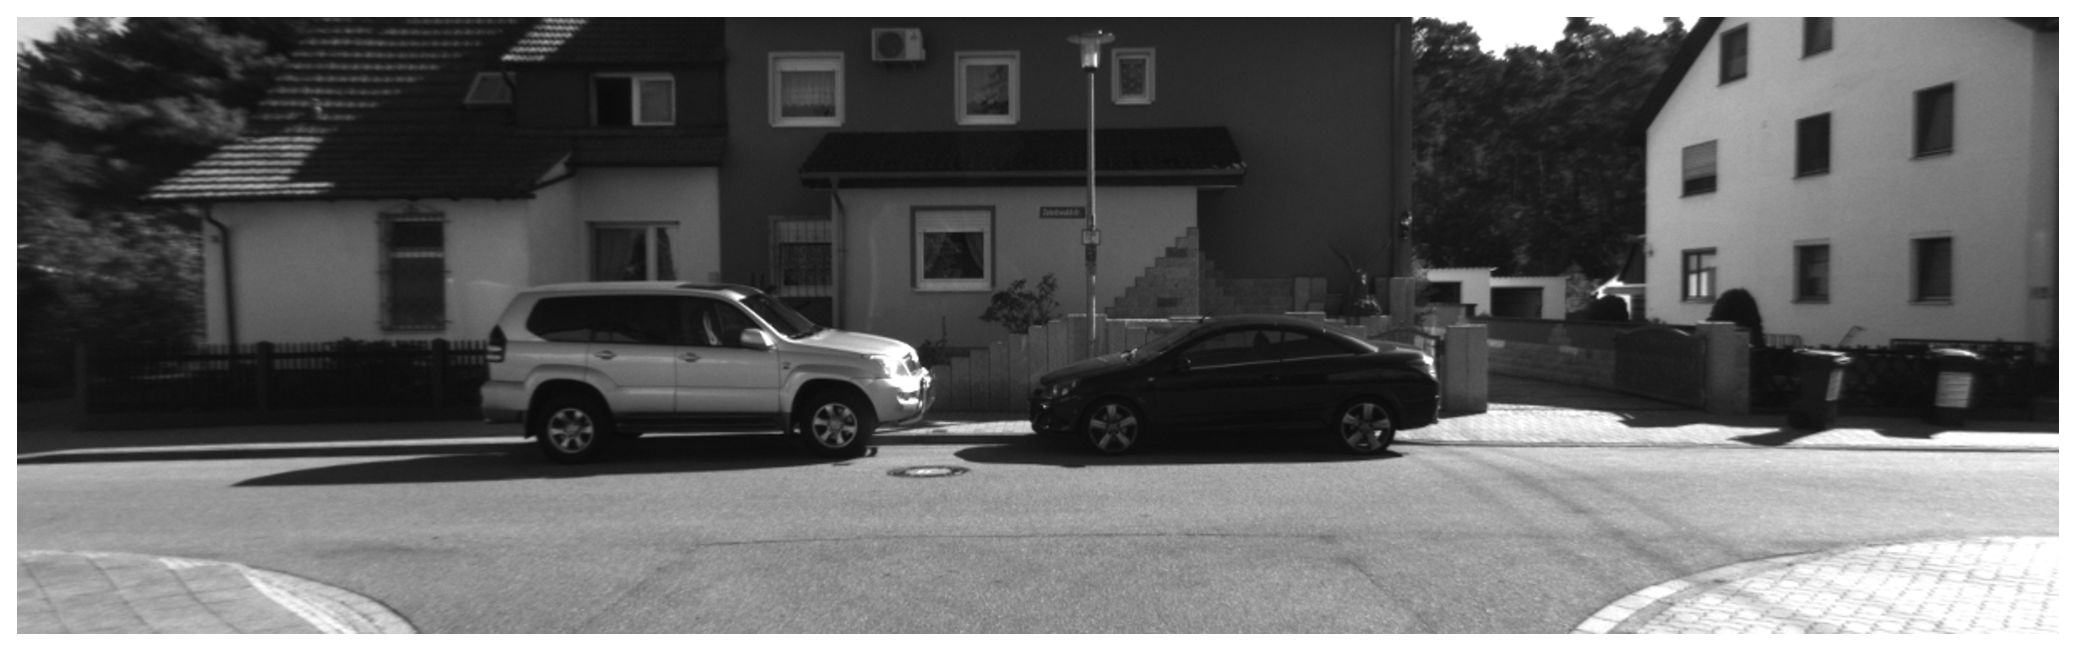
\includegraphics[scale=0.21]{000005L}}%
\subcaptionbox{Right image}
[.5\linewidth]{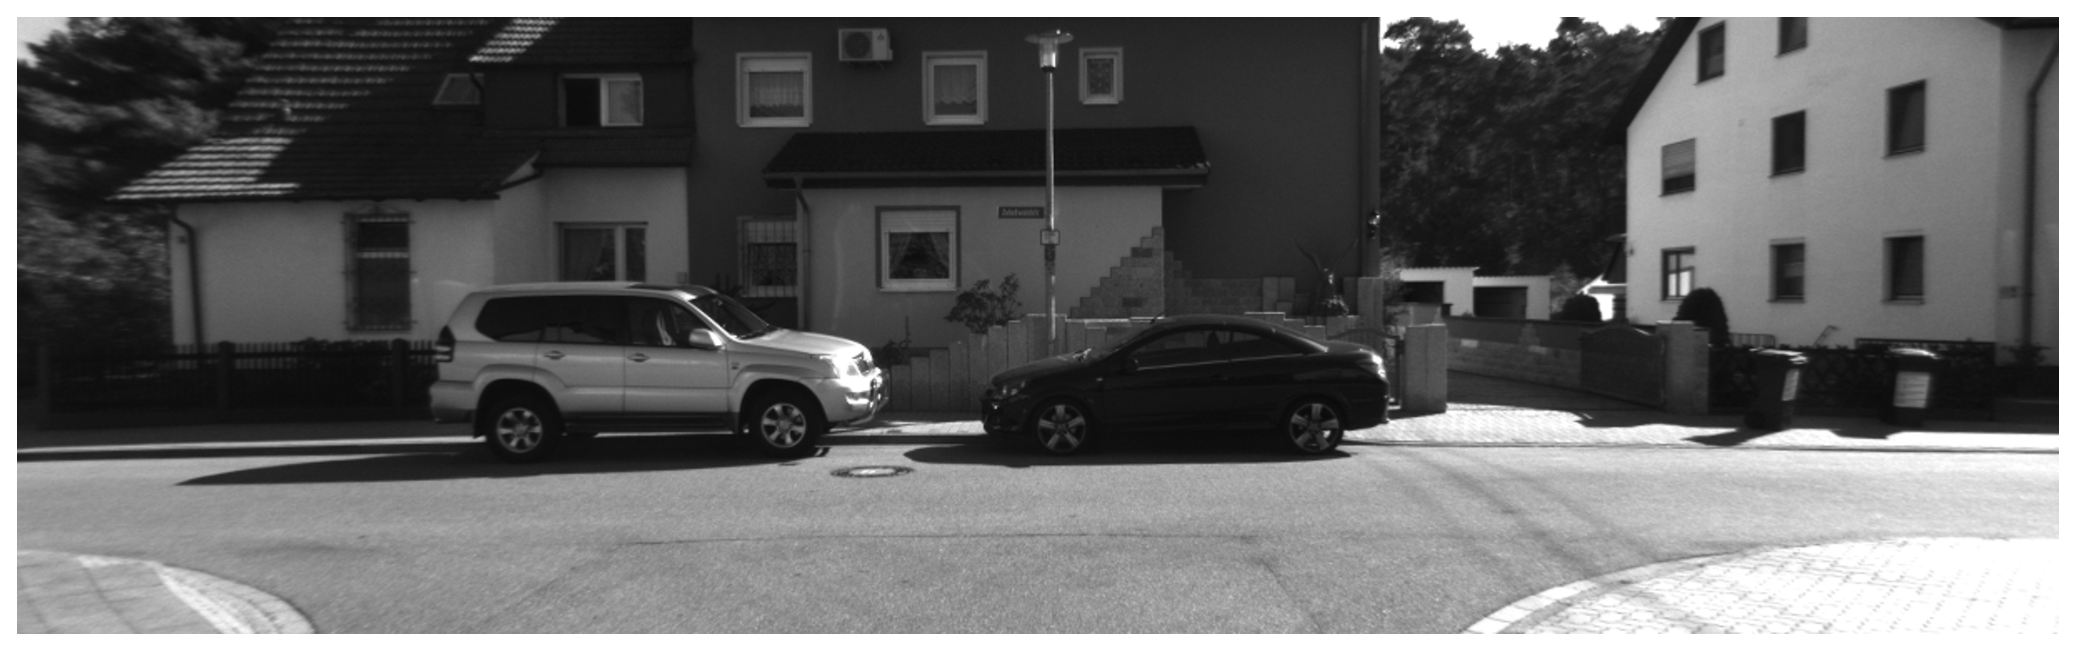
\includegraphics[scale=0.21]{000005R}}%
\caption{Sample stereo image from Kitti}
\label{fig:img5}
\end{figure}

\begin{figure}[H]
\centering
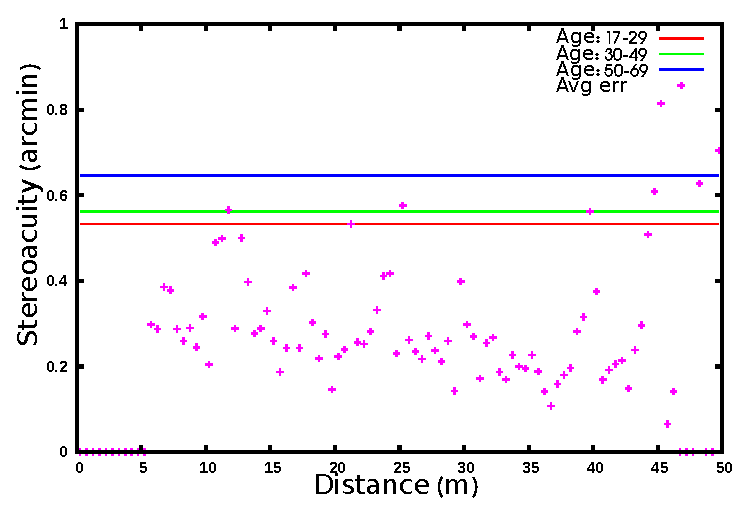
\includegraphics[scale=0.8]{sgbmimg5pix3msk}
\caption{Average disparity error over distance by SGBM}
\label{fig:imgmsk5}
\end{figure} 

\begin{figure}[H]
\centering
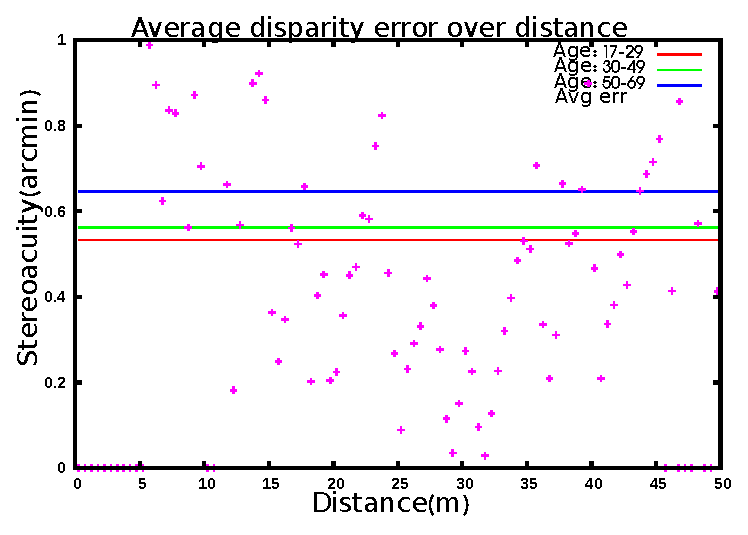
\includegraphics[scale=0.8]{adcimg5pix3msk}
\caption{Average disparity error over distance by ADCensus}
\label{fig:imgfull5}
\end{figure}

\noindent
The corresponding mask, figure \ref{fig:msk}; masked ground truth, figure \ref{fig:gtmsk}; and
the masked disparity images generated by SGBM and ADCensus, figure \ref{fig:5mdispsgb} and \ref{fig:5mdispadc} 
are shown below.

\begin{figure}[H]
\centering

\includegraphics[scale=0.35]{5msk}
\caption{The mask of depth edges and their surrounding regions}
\label{fig:msk}
\end{figure} 

\begin{figure}[H]
\centering

\includegraphics[scale=0.35]{5gt}
\caption{Masked ground truth}
\label{fig:gtmsk}
\end{figure} 

\begin{figure}[H]
\centering

\includegraphics[scale=0.35]{5mdispsgb}
\caption{Masked disparity by SGBM}
\label{fig:5mdispsgb}
\end{figure} 

\begin{figure}[H]
\centering

\includegraphics[scale=0.35]{5mdispadc}
\caption{Masked disparity by ADCensus}
\label{fig:5mdispadc}
\end{figure} 

\noindent
Figures \ref{fig:mskmapsgbm} and \ref{fig:mskmapadc} show the average results over all the disparity images for both SGBM and ADCensus, respectively.

\begin{figure}[H]
\centering
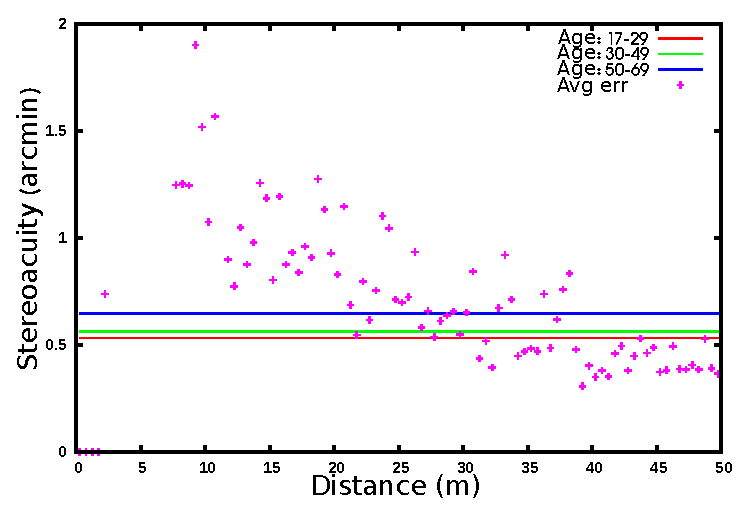
\includegraphics[scale=0.8]{sgbmmsk1000}
\caption{Average disparity error over all the images by SGBM}
\label{fig:mskmapsgbm}
\end{figure} 

\begin{figure}[H]
\centering
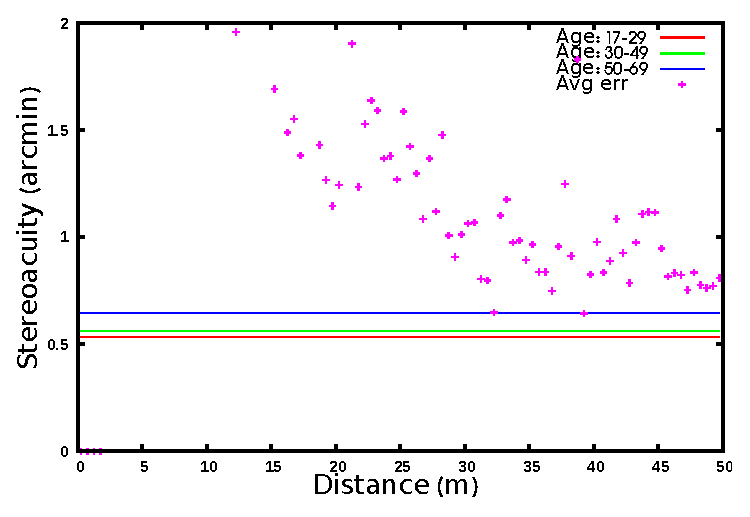
\includegraphics[scale=0.8]{adcenmsk1000}
\caption{Average disparity error over all the images by ADCensus}
\label{fig:mskmapadc}
\end{figure} 

As can be seen, the average results displayed in the previous plots, contain sparse points and 
do not demonstrate any consistent pattern. When we investigated the cause of this large variation, we found that in
the results of both algorithms, there are some disparity values which differ from the ground truth disparity 
by a considerable amount and yet have not been invalidated by the
algorithm. We assume that these types of outliers can be easily removed from the set by applying a post processing filter, or 
they will be culled out by the 3D renderer in the AR system in the end. 
%Therefore, we have added another filtering condition to our evaluation module is similar to the approach employed by the
%Kiiti and Middlebury stereo evaluation. 
In order to filter out the disparity values which largely differ from the ground truth disparity, we have integrated another 
step in our evaluation process. This step is similar to the strategy used in the Kitti and Middlebury evaluation models.
In this step, the estimated disparity error is initially compared to a more generally defined threshold, for instance a threshold of 3 pixels.
This comparison allows for only those values of disparity with an error less than or equal to the specified threshold to 
move on to the next steps of the evaluation. It should be noted in our design, the specified threshold is defined as a run-time variable. 

The additional filtering had a significant impact on the evaluation results. In fact, a consistent pattern was observed in the final plots after filtering out the
outliers with large differences. The results are displayed in
figures \ref{fig:mskmapsgbm} and \ref{fig:mskmapadc}.

\begin{figure}[H]
\centering
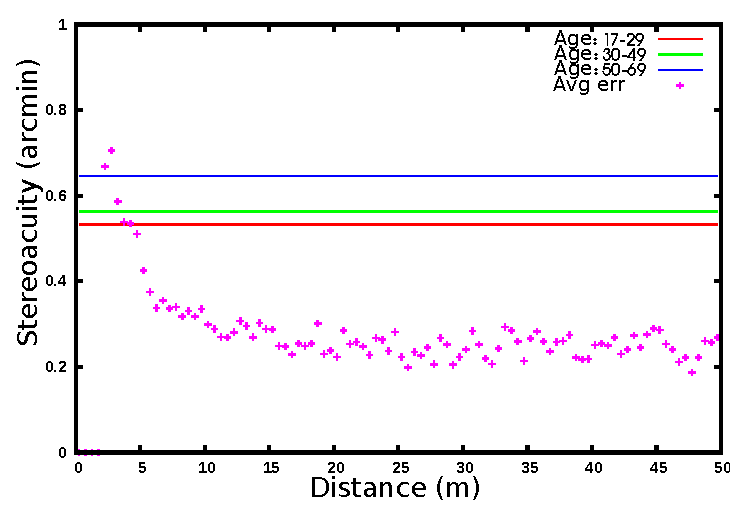
\includegraphics[scale=0.8]{sgbmmsk3}
\caption{Average disparity error over all the images by SGBM}
\label{fig:mskmapsgbm}
\end{figure} 

\begin{figure}[H]
\centering
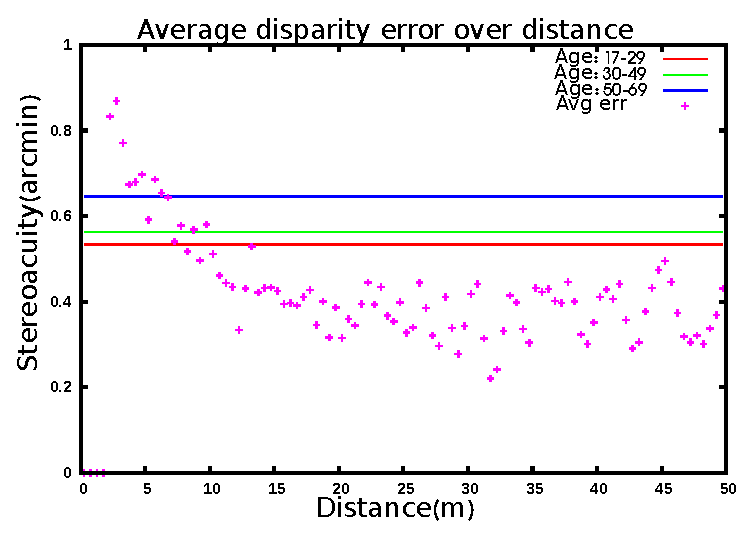
\includegraphics[scale=0.8]{adcenmsk3}
\caption{Average disparity error over all the images by ADCensus}
\label{fig:mskmapadc}
\end{figure} 

In these plots, a cross point below a stereoacuity threshold (straight lines) implies that the average error in the disparity values estimated 
by the stereo matching 
algorithm is imperceptible to the human visual system. However, a value higher than the threshold indicates that
the error cannot be ignored and should be resolved to achieve a better alignment between the virtual and the 
real world in the AR application of interest.

The zero values in the plots imply that either there is no object within the corresponding range or the disparity value estimated by the algorithm
is equal to the ground truth disparity; however, since the average of the results has been taken over all the images, it is more likely that 
the zero values indicate no object within the particular range.

As can be seen in the results, SGBM performs better in finding more accurate corresponding matches 
compared to ADCensus, as most of the error points fall below the standard stereoacuity lines. Moreover, the plots show that in both methods 
the significant amount of error
corresponds to the near field objects, within the first 5 meters. This range of the depth field can be considerably important in some applications,
such as the ones involving certain manipulative tasks.

\subsection{Depth edges and their surrounding area}
In order to examine the effect of evaluating certain regions of the disparity image instead of the whole image, 
we estimated the average error both for the masked areas and the whole disparity map. 
Results of SGBM are shown in figure \ref{fig:sgbmfull3} and \ref{fig:sgbmmsk3}.

\begin{figure}[H]
\centering
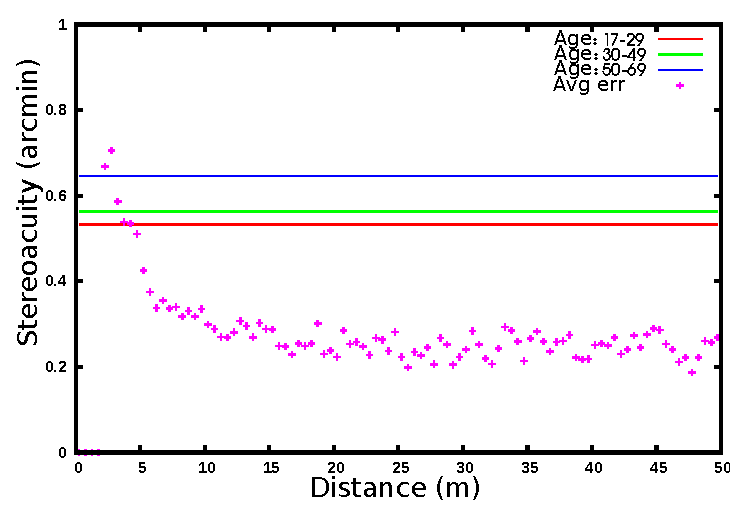
\includegraphics[scale=0.8]{sgbmmsk3}
\caption{Average disparity error over masked areas by SGBM}
\label{fig:sgbmmsk3}
\end{figure} 

\begin{figure}[H]
\centering
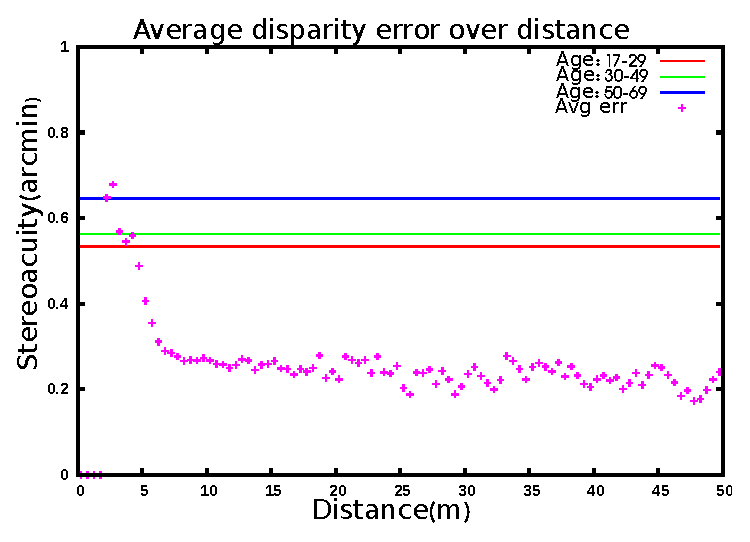
\includegraphics[scale=0.8]{sgbmfull3}
\caption{Average disparity error over all the regions by SGBM}
\label{fig:sgbmfull3}
\end{figure} 

The plots show that the average error over the masked regions, that is near the depth edges, is very similar to the results over the whole image. 
This may imply that there is no additional benefit in the inspection of these regions. 
However, this might be merely an indication of the performance of the selected algorithms, and can be better analyzed by evaluating more algorithms 
within our model.
In either case, we argue that, due to the importance of occlusion and areas near depth discontinuities to the HVS in AR applications, 
it is reasonable to focus more on the depth edges and their surroundings when designing or employing a stereo matching technique for an AR application.

\subsection{The average Outlier}
In this experiment the average number of outliers were measured for both algorithms. 
The values for both validity criteria mentioned in chapter \ref{chap:System} (valid pixels in the ground truth and generated disparity), were the same; therefore,
only one value is presented in the tables \ref{tab:outlmsk} and \ref{tab:outlfull} for each age group. \newline

%{\footnotesize
\begin{minipage}{0.8\linewidth}
\begin{center}
\captionof{table}{The average outliers for the masked regions}
\label{tab:outlmsk}
\begin{tabular}{ |c|c|c| }
\hline
\multicolumn{3}{ |c| }{Average outliers} \\
\hline
Algorithm & Age & Average Outlier \\ \hline
\multirow{4}{*}{SGBM} & 17-29 & 0.36 \\
& 30-49 & 0.35 \\
& 50-69 & 0.32 \\
& 70-83 & 0.23 \\ \hline
\multirow{4}{*}{ADCensus} & 17-29 & 0.52 \\
& 30-49 & 0.50 \\
& 50-69 & 0.47 \\
& 70-83 & 0.27 \\ \hline
\end{tabular}
\end{center}
\end{minipage} \newline \newline
%}

\begin{minipage}{0.8\linewidth}
\begin{center}
\captionof{table}{The average outliers for the whole images}
\label{tab:outlfull}
\begin{tabular}{ |c|c|c| }
\hline
\multicolumn{3}{ |c| }{Average outliers} \\
\hline
Algorithm & Age & Average Outlier \\ \hline
\multirow{4}{*}{SGBM} & 17-29 & 0.28 \\
& 30-49 & 0.27 \\
& 50-69 & 0.24 \\
& 70-83 & 0.16 \\ \hline
\multirow{4}{*}{ADCensus} & 17-29 & 0.56 \\
& 30-49 & 0.55 \\
& 50-69 & 0.52 \\
& 70-83 & 0.27 \\ \hline
\end{tabular}
\end{center}
\end{minipage} \newline

Results show that in both cases, the masked regions and the whole image, SGBM has less number of outliers than ADCensus, indicating that
SGBM generates a more accurate disparity map as perceived by the human visual system.
Furthermore, in SGBM the number of outliers over the masked regions are more than the outliers over the whole image, whereas in ADCensus the
opposite pattern is observed; that is the number of outliers over the masked regions are less than 
the whole image. This implies that ADCensus performs better in the areas of depth edges and their surroundings than other regions.
Therefore, it is better to be employed in applications, 
where preserving the object boundaries and occluded areas
is more important than the other regions in the image, such as 3D layering of objects \textbf{(NOTE CHECK THE CORRECT TERM)}. However, this metric per se
cannot be an indicator of a proper solution for any target application and should be considered along with the other
relevant metrics. 

\subsection{The average disparity error}
The average disparity error have also been estimated in the evaluation process for both pixel validity criteria. However, the resulting values
were similar for both cases, and therefore, only one number is reported in the following table for this metric. \newline

\begin{minipage}{0.8\linewidth}
\begin{center}
\captionof{table}{The average outliers for the whole images}
\label{tab:avgerr}
\begin{tabular}{ |c|c|c| }
\hline
\multicolumn{3}{ |c| }{Average disparity error} \\
\hline
Algorithm & Region & error \\ \hline
\multirow{2}{*}{SGBM} & Full & 6.58 \\
& Masked & 7.81 \\ \hline
\multirow{2}{*}{ADCensus} & Full & 4.49 \\
& Masked & 4.74 \\ \hline
\end{tabular}
\end{center}
\end{minipage} \newline

As can be seen, ADCensus results in less average disparity error than SGBM. This difference is likely caused by the various refinement steps
implemented in ADCensus algorithm which do not exist in SGBM.
As a result, despite the larger number of outliers in ADCensus than SGBM as measured in the previous experiments,
ADCensus attempts to decrease the difference between the resulting disparity value and the ground truth disparity, thus generating a smoother disparity patches
within different regions of the image.

\subsection{Real-time execution}
In another experiment we estimated the average execution time for both algorithms. Results show that the average execution time over all the images 
for SGBM and ADCensus are $0.54$ and $272.82$ seconds, respectively.
Considering the requirements of having an interactive real-time AR system \cite{hertz00}, the processing time of each frame should not be more than 0.06-0.08 seconds.
Although the current implementation of SGBM could be used when the real world scene remains stable for approximately one second, it can be safely concluded that
none of these algorithms meet the requirements of a real-time interactive system.
This suggests that the GPU-based solutions are better techniques to achieve the processing speed required for the real-time 
interactive applications of AR.

\subsection{Effect of Refinement}
In this experiment, we intended to study the effect of the post processing steps, also referred to as the \textit{refinement steps}, 
in the stereo algorithms on the accuracy of the results in our evaluation criteria. 
To this end, we modified our implementation 
of the ADcensus algorithm by taking out each independant refinement step, generating the disparity results for the image pairs, and evaluating the results.
The results over both the masked and the whole image are shown below.


Next, we will review the hypotheses mentioned earlier in this chapter and will discuss their validity based on our experiments and their results.
